%%% Results %%%
\chapter{Results} \label{ch:results}
This chapter evaluates the result of endorsement model as presented in section
~\ref{ch:method} by using interaction graph on existing dataset. Results will
be presented along with the discussion of measurement metrics and analyzed to
see if the requirements mentioned in section ~\ref{ch:UserStories} are met.  
%%%%%%%%%%%%%%%%%%%%%%%%%%%%%%%%%%%%%%%%%%%%%%%%%%%%%%%%%%%%%%%

%%%%%%%%%%%%%%%%%%%%%%%%%%%%%%%%%%%%%%%%%%%%%%%%%%%%%%%%%%%%%%%
\section{Interaction graph}
In order to simulate the interaction graph, existing dataset from SNAP
\cite{snapnets} was used. The dataset was extracted from Bitcoin Alpha trust
\footnote{https://alphabtc.com/blockchain/}
weighted signed network which was essentially a who-trusts-whom network of
people that trade on Bitcoin Alpha platform. Participants on this network rated
each other on a scale of -10 to +10 where negative value represented total
distrust whereas positive value represented total trust. It consists of 3,783
nodes that made 24,186 edges out of which 93\% of the edges were marked as
positive edges\cite{kumar2016edge}. 

\begin{figure}[h]
	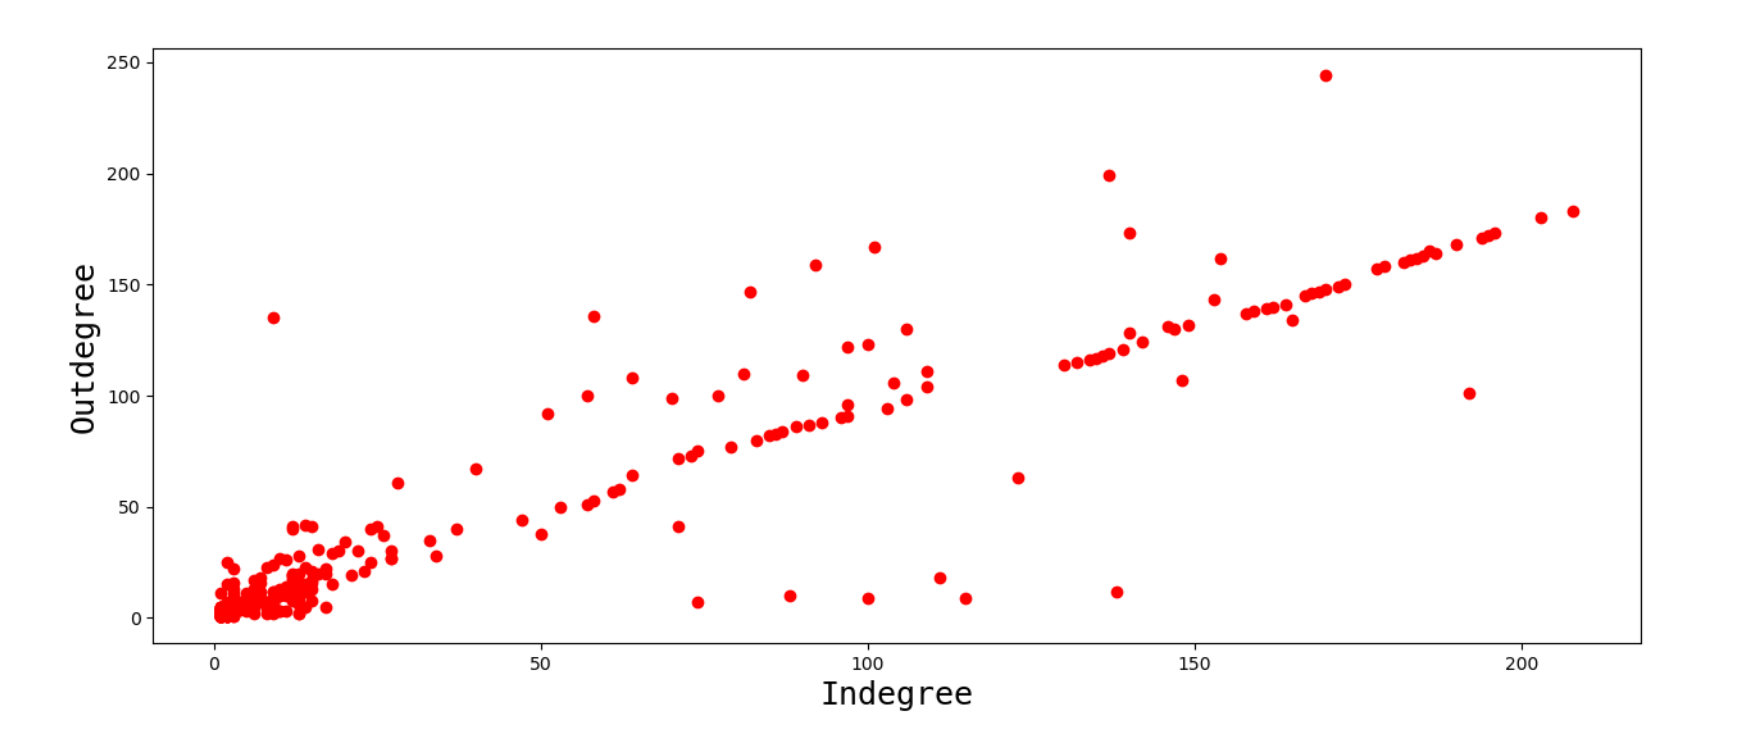
\includegraphics[width=0.95\textwidth]{Images/in_out.eps}
	\caption{Given Vs. Received}
	\label{inOut}
\end{figure}

The available information in the dataset for all the nodes was source, target,
rating, and timestamp. All of these are essential information for endorsement
network. The direction of endorsement is based on the source and target
information. For the endorsement relation, all the edges with a rating above
five were considered. The timestamp is also essential information when using a
network anomaly detection algorithm such as net flow rate convergence(cite). An
interaction subgraph can be seen in figure ~\ref{subgraph} that shows the node
with an id of '561' and all its relations. The distribution of incoming and
outgoing connections of each node can be seen in figure ~\ref{inOut}. 

\begin{figure}[h]
	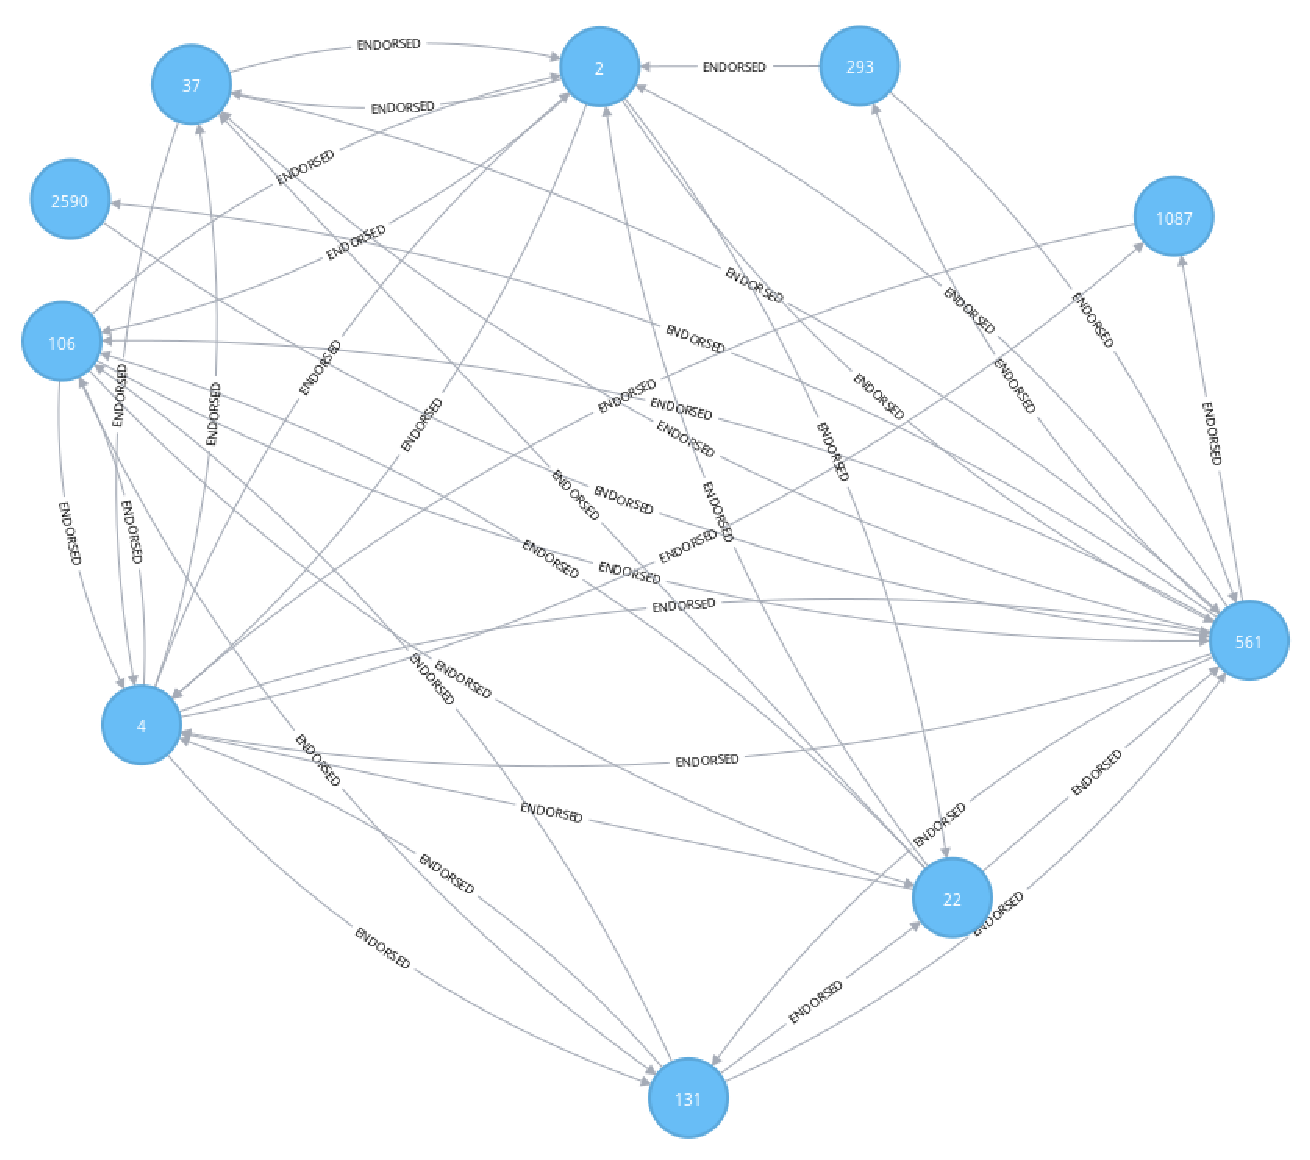
\includegraphics[width=0.9\textwidth]{Images/graph_Node561.eps}
	\caption{Interaction subgraph} 
	\label{subgraph}
\end{figure}














%\section{Analysis}
%\section{Measurement}
%\section{Comparison}
%\section{first section} \label{sec:sectionlabel}

% Presentation of results and case-study data 
% An application of the methodology is unfolded and results are presented using for example via Charts, Diagrams, Figures and Tables 
% The work is conducted in accordance with the method described earlier. Results are presented in an analytical way.
